% Compile from the project root with tectonic COURSE_PROJECT_SLIDES_FINAL_V2.tex.
% Rebuild figures with python scripts/build_slide_assets.py.
% The 20 numbered frames have a target running time of 18 minutes.
% Speaker notes are embedded with \note{} and hidden in the audience PDF.
\documentclass[aspectratio=169,11pt]{beamer}
\usepackage[T1]{fontenc}
\usepackage{lmodern,amsmath,amssymb,booktabs}
\usepackage{tikz}
\usetikzlibrary{positioning,arrows.meta,calc}
\usefonttheme{professionalfonts}
\definecolor{navy}{HTML}{16364A}
\definecolor{teal}{HTML}{007F83}
\definecolor{orange}{HTML}{C45A13}
\definecolor{muted}{HTML}{576574}
\setbeamercolor{normal text}{fg=navy,bg=white}
\setbeamercolor{structure}{fg=teal}
\setbeamercolor{frametitle}{fg=navy}
\setbeamercolor{block title}{fg=white,bg=navy}
\setbeamercolor{block body}{fg=navy,bg=navy!5}
\setbeamerfont{frametitle}{size=\Large,series=\bfseries}
\setbeamerfont{title}{size=\LARGE,series=\bfseries}
\setbeamertemplate{navigation symbols}{}
\setbeamertemplate{itemize items}[circle]
\setbeamersize{text margin left=8mm,text margin right=8mm}
\setbeamertemplate{footline}{%
  \hspace{8mm}\textcolor{muted}{\scriptsize\insertsectionhead}
  \hfill\textcolor{muted}{\scriptsize\insertframenumber/\inserttotalframenumber}
  \hspace{8mm}\vspace{3mm}}
\setbeamertemplate{frametitle}{\vspace{3mm}\insertframetitle\par\vspace{2mm}}
\setbeameroption{hide notes}
\newcommand{\norm}[1]{\lVert #1\rVert_2}
\newcommand{\tf}{f_\phi}
\newcommand{\source}[1]{\par\vfill{\color{muted}\tiny #1}}
\title{Stability and Information Sensitivity\\in Transformer In-Context Inverse Learning}
\author{Fei Zhang}
\institute{University of Waterloo\\CS 886}
\date{November 2026}


\begin{document}
\section{Motivation}

\begin{frame}[plain]
\vfill
{\usebeamerfont{title}\inserttitle\par}
\vspace{6mm}
{\large Fei Zhang\par}
\vspace{2mm}
{\color{muted}University of Waterloo\quad CS 886\par}
\vspace{7mm}
{\color{teal}\large Can a stable Transformer use the one record that identifies a task?}
\vfill
\note{Target time 25 seconds, cumulative 0:25.
The question for this talk is what happens when almost all the useful
information about one parameter sits in a single observation. We examine
a frozen Transformer, first through a simple example and two complementary
bounds, then through controlled inverse-learning experiments.}
\end{frame}

\begin{frame}{When should one observation change the answer?}
\begin{columns}[T,onlytextwidth]
\column{.47\textwidth}
{\large Ordinary replacement}
\vspace{3mm}

A different record from the same task.

\[
\theta'=\theta
\]

A small prediction change can accompany accurate recovery.
\column{.47\textwidth}
{\large Identifying replacement}
\vspace{3mm}

A record that distinguishes two tasks.

\[
\theta'\ne\theta
\]

Accurate recovery requires the prediction to change.
\end{columns}
\vspace{6mm}
\begin{block}{Research question}
Can a Transformer remain stable while responding enough to the observations
that determine the correct task parameters?
\end{block}
\note{Target time 40 seconds, cumulative 1:05.
Small sensitivity can mean different things. If I replace an observation
with another from the same task, the correct parameters stay the same,
so an unchanged prediction can be exactly right. If a replacement
distinguishes two different tasks, the correct answer changes.
An estimator that stays almost unchanged may then be wrong.
Our question is whether the model makes that distinction.
To make the distinction concrete, consider a line with an unknown slope.}
\end{frame}

\begin{frame}{A single record can determine the slope}
\begin{columns}[c,onlytextwidth]
\column{.52\textwidth}
\[
y=bx
\]
{\small\setlength{\tabcolsep}{4pt}
\begin{tabular}{lcc}
\toprule
& Context A & Context B\\
\midrule
Shared \(m-1\) records & \((0,0)\) & \((0,0)\)\\
Last record & \((1,1)\) & \((1,2)\)\\
\midrule
Correct slope & \(b=1\) & \(b=2\)\\
\bottomrule
\end{tabular}
}
\vspace{4mm}

Each context identifies its slope.

Adding copies of \((0,0)\) supplies no new slope information.
\column{.44\textwidth}
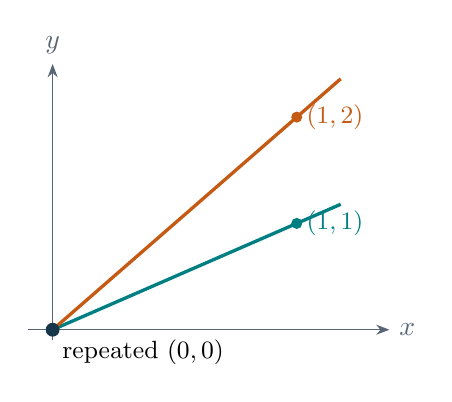
\begin{tikzpicture}[x=3.1cm,y=1.35cm,>=Stealth]
\draw[->,muted] (-.1,0)--(1.38,0) node[right]{\(x\)};
\draw[->,muted] (0,-.1)--(0,2.5) node[above]{\(y\)};
\draw[teal,very thick] (0,0)--(1.18,1.18);
\draw[orange,very thick] (0,0)--(1.18,2.36);
\fill[teal] (1,1) circle (2pt);
\fill[orange] (1,2) circle (2pt);
\fill[navy] (0,0) circle (2.5pt);
\node[teal,right,font=\small] at (1,1){\((1,1)\)};
\node[orange,right,font=\small] at (1,2){\((1,2)\)};
\node[below right,font=\small] at (0,0){repeated \((0,0)\)};
\end{tikzpicture}
\end{columns}
\vspace{4mm}
{\color{teal}\large Only one record changes, but the correct answer changes by 1.}
\note{Target time 65 seconds, cumulative 2:10.
Both contexts contain the same repeated zeros. Every line through
the origin is consistent with those zeros, so they tell us nothing
about the slope. The last record supplies the slope: one in A and
two in B. Each complete context has a unique correct answer.
Now imagine adding a thousand more copies of the zero record.
The answer still depends on that last observation just as strongly.
This is the example to keep in mind throughout the theory.
We will compare how much an architecture can respond with how much
accurate recovery requires it to respond.}
\end{frame}

\begin{frame}{Possible response and required response}
Let \(\Delta=\norm{f(S)-f(S')}\) and \(D=\norm{\theta-\theta'}\).
\vspace{4mm}
\begin{columns}[T,onlytextwidth]
\column{.47\textwidth}
{\large Theorem 1: architecture}
\[
\Delta\le C/m
\]
How much can a fixed encoder change when one record changes?
\column{.47\textwidth}
{\large Theorem 2: recovery}
\[
\Delta\ge D-2\epsilon
\]
How much must any estimator change if both errors are at most \(\epsilon\)?
\end{columns}
\vspace{7mm}
{\color{teal}\large The same response \(\Delta\) must support accurate task recovery.}
\par\vspace{2mm}
\small KKT gives a controlled setting where we can check which records identify the task.
\source{The first bound adapts established Transformer stability reasoning.
The second follows from the triangle inequality.}
\note{Target time 40 seconds, cumulative 2:50.
There are two separate questions. Theorem one gives a ceiling on
the response permitted by the architecture. Theorem two gives a
floor on the response required for accuracy. Delta is the same
prediction difference in both statements. D is the distance between
the correct parameters. Neither statement says that a smaller
response is always better. To study this tension in a structured setting, we consider an inverse
optimization problem where KKT conditions characterize which observations
identify the unknown task parameters. This provides a controlled testbed
for Transformer recovery. It does not introduce a separate electricity-market
research question.}
\end{frame}

\section{Methodology}
\begin{frame}{Learning cost parameters from dispatch observations}
\begin{columns}[T,onlytextwidth]
\column{.49\textwidth}
{\large A controlled testbed}
\[
\min_{\substack{x_1+x_2=d\\0\le x_i\le1}}
\sum_{i=1}^2\left(a_ix_i+\tfrac12b_ix_i^2\right).
\]
Unknown costs:
\[
\theta=(a_1,b_1,a_2,b_2).
\]
Observed record:
\[
z_t=(d_t,x_{1t},x_{2t},\lambda_t,s_{1t},s_{2t}).
\]
\column{.47\textwidth}
{\large Interior KKT information}\par\vspace{1mm}
For an interior generator, KKT gives
\[
\lambda_t=a_i+b_ix_{it}.
\]
KKT makes the identifying information explicit.

\vspace{3mm}
Two distinct interior outputs identify the two coefficients.

\vspace{3mm}
A bound status supplies an inequality.
\end{columns}
\vspace{1mm}
\[
S_m
\ \xrightarrow{\ \text{2-layer Transformer}\ }\ H
\ \xrightarrow{\ \text{mean pooling and head}\ }\ \widehat\theta.
\]
\source{Supervised source-task training. Weights stay fixed on unseen tasks.
Two unit-capacity generators, positive bounded cost slopes.}
\note{Target time 75 seconds, cumulative 4:05.
Inverse optimization is useful here because we can explicitly check
what each record tells us about the unknown task. Our objective is to
understand Transformer recovery, rather than demonstrate superiority over
classical inverse optimization. Each synthetic task has four unknown cost coefficients. For a given
demand we observe optimal generator outputs, a clearing price, and
whether each output is at a bound. The price equals marginal cost
for an interior generator. This produces exactly the affine equation
from the motivating example. Two different interior outputs identify
that generator's intercept and slope. Bound observations instead
give one-sided inequalities. A two-layer Transformer reads complete
market records, averages its final token states, and predicts four
cost coefficients through a bounded head. We train it on labeled
source tasks, then freeze it on new tasks. The question is how its
context response relates to the information in these equations.
We first establish an architectural upper bound.}
\end{frame}

\begin{frame}{Theorem 1: a fixed encoder has a \(C/m\) response bound}
\begin{block}{Encoder replacement stability}
Fix finite weights and depth, bounded records, full attention,
a mean-pooled Lipschitz readout, and positive LayerNorm epsilon.
Then a finite \(C\), independent of \(m\), satisfies
\[
\boxed{\norm{f_\phi(S_m)-f_\phi(S_m')}\le C/m}
\]
for any two contexts differing in one record, in exact arithmetic.
\end{block}
\vspace{3mm}
\begin{itemize}
\setlength{\itemsep}{2mm}
\item The same frozen model processes every context length.
\item The worst-case response tends to zero as \(m\) grows.
\item Affine record embeddings, no positional encoding, and no attention mask.
\end{itemize}
\source{Architecture-specific adaptation of bounded-attention stability
arguments, including Li et al. (2023).}
\note{Target time 50 seconds, cumulative 4:55.
The theorem compares one fixed model across lengths. It does not retrain
a new model as m increases. Under the stated assumptions, every
single-record replacement has a response bounded by C divided by m.
Because C stays fixed, the bound eventually tends to zero.
This is a worst-case upper bound, rather than a claim that every
measured response lies exactly on an inverse-length curve.
The actual implementation uses an affine 10-to-64 record embedding,
four heads, two post-residual normalization blocks per layer, ReLU
feedforward maps and zero dropout. The LayerNorm epsilon is positive.
There is no positional embedding or sequence-dependent mask.
Bounded records and finite maps bound all hidden rows at fixed depth,
independently of context length. The proof explains dilution and C.}
\end{frame}

\begin{frame}{Proof step 1: one changed row and bounded attention}
\small
\setlength{\abovedisplayskip}{3pt}
\setlength{\belowdisplayskip}{3pt}
\setlength{\abovedisplayshortskip}{2pt}
\setlength{\belowdisplayshortskip}{2pt}
\begin{columns}[T,onlytextwidth]
\column{.46\textwidth}
\textbf{Track the average token change}
\[
e_i=\norm{h_i-h_i'},\qquad
\bar e=\frac1m\sum_{i=1}^m e_i.
\]
Only one embedded record changes:
\[
\boxed{\bar e^{(0)}\le A/m.}
\]
\small An individual row can change substantially.
The average tracks how this change spreads through attention.
\column{.50\textwidth}
\textbf{Fixed maps on bounded states}
\small
\[
\begin{aligned}
q_i&=W_Qh_i+b_Q,\\
k_j&=W_Kh_j+b_K,\\
v_j&=W_Vh_j+b_V,\\
s_{ij}&=q_i^\top k_j/\sqrt{d_k}.
\end{aligned}
\]
Finite weights and uniformly bounded hidden rows imply
\(\lvert s_{ij}\rvert,\lvert s'_{ij}\rvert\le B\), independent of \(m\).
\end{columns}
\vspace{2mm}
\[
p_{ij}=\frac{e^{s_{ij}}}{\sum_k e^{s_{ik}}}
\le\frac{e^B}{me^{-B}}
=\boxed{\frac{e^{2B}}m}.
\]
{\color{teal}\small Bounded logits limit the weight of any individual record as the context grows.}
\source{\(A\) bounds a single embedded-row change; fixed affine biases are included.
State bounds follow inductively from bounded records and fixed finite maps.}
\note{Target time 60 seconds, cumulative 5:55.
We track the average token difference because attention can move the
initial change into many rows. One row may change a lot, but immediately
after embedding only that row differs. Its contribution to the average
is at most A divided by m. Queries, keys and values are fixed affine
maps of bounded states. Their norms, and hence the scores, have bounds
independent of context length. In softmax the largest possible numerator
is exp B. Every denominator term is at least exp minus B, and there are
m of them. This gives exp two B divided by m. That limits each record's
attention weight. We must still check both changed values and changed
weights, because replacing a record can affect both.}
\end{frame}

\begin{frame}{Proof step 2: control value changes and weight changes}
\fontsize{9.5}{11.2}\selectfont
\setlength{\abovedisplayskip}{2pt}
\setlength{\belowdisplayskip}{2pt}
\setlength{\abovedisplayshortskip}{1pt}
\setlength{\belowdisplayshortskip}{1pt}
For one head, \(\operatorname{Attn}_i(H)=\sum_jp_{ij}v_j\). Split its change:
\[
\operatorname{Attn}_i(H)-\operatorname{Attn}_i(H')
=
\underbrace{\textstyle\textstyle\sum_jp_{ij}(v_j-v_j')}_{\textcolor{teal}{\text{value change}}}
+
\underbrace{\textstyle\sum_j(p_{ij}-p_{ij}')v_j'}_{\textcolor{orange}{\text{weight change}}}.
\]
\vspace{-3mm}
\begin{columns}[T,onlytextwidth]
\column{.42\textwidth}
{\color{teal}\textbf{Value change}}
\[
\|v_j-v_j'\|_2\le\|W_V\|e_j,
\]
\[
\left\|\textstyle\sum_jp_{ij}(v_j-v_j')\right\|_2
\le\|W_V\|e^{2B}\bar e.
\]
\column{.55\textwidth}
{\color{orange}\textbf{Weight change: queries and keys move}}
\[
|s_{ij}-s_{ij}'|\le c_qe_i+c_ke_j.
\]
\[
\begin{aligned}
J(p)&=\operatorname{diag}(p)-pp^\top,\\
\textstyle\sum_k|J_{kj}|&=2p_j(1-p_j)\le 2e^{2B}/m.
\end{aligned}
\]
Integrate along the score segment (Backup A):
\[
\|p_i-p_i'\|_1\le2e^{2B}(c_qe_i+c_k\bar e).
\]
\end{columns}
\vspace{1mm}
Bounded values give
\(\|v_j'\|_2\le V_0\ \Longrightarrow\
\|\sum_j(p_{ij}-p_{ij}')v_j'\|_2\le V_0\|p_i-p_i'\|_1.\)
\vspace{-1mm}
\[
\begin{aligned}
\|\operatorname{Attn}_i(H)-\operatorname{Attn}_i(H')\|_2
&\le\alpha e_i+\beta\bar e,\\
\textstyle\frac1m\sum_i\|\operatorname{Attn}_i(H)-\operatorname{Attn}_i(H')\|_2
&\le(\alpha+\beta)\bar e=L_{\rm att}\bar e.
\end{aligned}
\]
{\color{teal}Attention spreads change; average amplification stays bounded independently of \(m\).}
\source{Constants are independent of \(m\); fixed multihead projections only change these constants.}
\note{Target time 90 seconds, cumulative 7:25.
The attention output can change in two ways. First hold the old
weights fixed and change the values. The affine value map cancels
its bias in the difference. Multiplying each row difference by an
attention weight bounded by exp two B over m produces a constant
times the average input change. The second term keeps the new
values fixed and changes the attention weights. Bounded values
turn this into a probability-vector difference in the one norm.
Both the query of row i and the keys of other rows can move.
Their score changes therefore have a local e i term and a key e j
term. The displayed Jacobian column sum bounds how changing one
score changes the full probability vector. Integrating along the
score segment gives a local query term plus the average key change.
Combining the two components gives alpha times e i plus beta times
the average. Averaging over i converts the local term into another
average term. This is the crucial step: attention can spread change,
but cannot amplify the average by a factor growing with m.
Fixed head concatenation and output projection preserve this form.
We can now compose the remaining encoder operations.}
\end{frame}

\begin{frame}{Proof step 3: compose the blocks, pooling and head}
\small
\setlength{\abovedisplayskip}{3pt}
\setlength{\belowdisplayskip}{3pt}
\setlength{\abovedisplayshortskip}{2pt}
\setlength{\belowdisplayshortskip}{2pt}
\begin{columns}[T,onlytextwidth]
\column{.43\textwidth}
\textbf{Finite rowwise and residual factors}
\[
\begin{array}{ll}
\text{Attention + residual:}&1+L_{\rm att},\\[2mm]
\text{FF + residual:}&1+\|W_2\|\|W_1\|,\\[2mm]
\text{LayerNorm:}&
\displaystyle L_{\rm LN}\le\frac{\|\gamma\|_\infty}{\sqrt\eta}.
\end{array}
\]
ReLU gives \(L_\sigma=1\); \(\eta>0\).
Both LayerNorm maps enter each layer's factor \(L_\ell\).
\column{.53\textwidth}
\textbf{Compose complete encoder layers}
\[
\bar e^{(\ell)}\le L_\ell\bar e^{(\ell-1)}.
\]
\[
\bar e^{(L)}
\le\left(\prod_{\ell=1}^{L}L_\ell\right)\bar e^{(0)}
\le\frac Am\prod_{\ell=1}^{L}L_\ell.
\]
\textbf{Mean pooling cannot increase the average}
\[
\left\|\frac1m\sum_i(h_i^{(L)}-h_i'^{(L)})\right\|_2
\le\bar e^{(L)}.
\]
\end{columns}
\vspace{1mm}
\[
\Delta\le L_{\rm head}\bar e^{(L)}
\le\frac{A L_{\rm head}\prod_\ell L_\ell}{m}
=\frac Cm,\qquad
\boxed{C=A L_{\rm head}\prod_\ell L_\ell.}
\]
{\color{teal}Fixed depth preserves the initial \(O(1/m)\) average perturbation rate.}
\par\vspace{1mm}
\textcolor{orange}{Norm certificate: \(\log_{10}C=616.5\)--\(708.9\);
vacuous at measured \(m\le64\).}
\source{Matrix norms are Euclidean operator norms.
Backup B proves the LayerNorm bound. The sigmoid/box head is Lipschitz.}
\note{Target time 60 seconds, cumulative 8:25.
The attention result now supplies one finite factor. Adding its
residual contributes one plus that factor. The feedforward block
uses ReLU, which is one-Lipschitz, so its residual factor is one plus
the product of the two weight norms. Each positive-epsilon LayerNorm
also has a finite factor; both normalizations are included in each
complete layer bound. Repeating the recurrence multiplies these
factors but leaves the initial one over m intact. Mean pooling is
bounded by the average row difference. Finally the prediction head
contributes its Lipschitz constant. Everything in the numerator is
C and stays independent of context length. This proves an eventual
rate. Its norm-based certificate is enormous and vacuous at measured
lengths. We next ask how much response accuracy requires, independently
of this loose numerical ceiling.}
\end{frame}

\begin{frame}{Theorem 2: recovery requires enough response}
For any estimator, write
\[
D=\norm{\theta-\theta'},\quad
\Delta=\norm{f(S)-f(S')},\quad
e_A=\norm{\theta-f(S)},\quad e_B=\norm{\theta'-f(S')}.
\]
The triangle inequality along the two predictions gives
\[
\underbrace{\norm{\theta-\theta'}}_{D}
\le
\underbrace{\norm{\theta-f(S)}}_{e_A}
+
\underbrace{\norm{f(S)-f(S')}}_{\Delta}
+
\underbrace{\norm{f(S')-\theta'}}_{e_B}.
\]
Thus
\[
\boxed{\max(e_A,e_B)\ge\tfrac12(D-\Delta)_+.}
\]
If both errors are at most \(\epsilon\), then \(\boxed{\Delta\ge D-2\epsilon}\).
\vspace{4mm}

{\color{teal}In the slope example, \(D=1\).
Errors at most \(0.1\) require a response of at least \(0.8\).}
\source{A generic geometric necessary condition. It applies to any estimator
and supplies the recovery side of the argument.}
\note{Target time 80 seconds, cumulative 9:45.
Return to slopes one and two. Accurate predictions must move from
near one to near two. The theorem formalizes this requirement.
Go from the first true parameter to its prediction, then to the
second prediction, then to the second true parameter. These three
lengths must sum to at least the distance between the truths.
If the middle segment is short, the endpoint errors must supply
the remaining distance. At least one error is therefore at least
half of D minus Delta. This does not mean both endpoints must be
wrong: one could be exact and the other very inaccurate.
Equivalently, errors below epsilon on both sides require a response
of at least D minus two epsilon. With D equal to one and epsilon
equal to one tenth, that is a response of at least eight tenths.
This proof uses only the triangle inequality and is not
Transformer-specific.}
\end{frame}

\begin{frame}{Corollary: a worst-case limitation of stable recovery}
\small
Suppose, for every \(m\ge2\), neighboring contexts \(S_A^{(m)},S_B^{(m)}\)
each identify their own fixed task, with target separation \(D>0\).
For one fixed encoder satisfying Theorem 1,
\[
\boxed{\max\{e_A^{(m)},e_B^{(m)}\}
\ge \frac12\left(D-\frac Cm\right)_+.}
\]
Consequently,
\[
\boxed{\liminf_{m\to\infty}
\max\{e_A^{(m)},e_B^{(m)}\}\ge D/2.}
\]
\begin{itemize}
\setlength{\itemsep}{1.5mm}
\item One identifying record differs. Repeat the common background \(m-1\) times.
\item Each endpoint stays identifying and \(D\) stays fixed.
\item In the slope example, repeated zeros add no slope information and \(D=1\).
\end{itemize}
\source{Proof: substitute Theorem 1 into Theorem 2, then take the liminf.
Worst-case existence, not an average-case error floor.
The numerical certificate is vacuous at measured lengths.}
\note{Target time 45 seconds, cumulative 10:30.
This corollary is the central theoretical result of the project.
For each length, use two individually identifying contexts with only
one differing record and fixed target separation. Apply the two bounds.
The finite-length result follows immediately, and taking the limit inferior
gives a floor of D over two on the larger endpoint error.
The slope example supplies intuition: more zero records add no identifying
information. This is an existence construction, not an average-case
error floor, and the numerical certificate is vacuous at our tested lengths.
We next construct the same situation using valid dispatch observations.}
\end{frame}

\begin{frame}{The identifying pair exists in valid dispatch data}
\begin{center}
\begin{tabular}{lcc}
\toprule
& Task A & Task B\\
\midrule
Each generator's \((a_i,b_i)\)&\((1.6,1.0)\)&\((1.2,1.8)\)\\
Shared record at \(d=1\)&\((0.5,0.5,2.10)\)&\((0.5,0.5,2.10)\)\\
Identifying record at \(d=1.6\)&\((0.8,0.8,2.40)\)&\((0.8,0.8,2.64)\)\\
\bottomrule
\end{tabular}
\end{center}
\vspace{3mm}
\begin{itemize}
\setlength{\itemsep}{2mm}
\item Records list \((x_1,x_2,\lambda)\). All outputs are interior.
\item Repeat the shared record \(m-1\) times. The contexts differ in exactly one price.
\item Two distinct outputs identify each cost; \(D=\sqrt{1.6}\) stays fixed for all \(m\ge2\).
\end{itemize}
\vspace{3mm}
{\color{teal}Each context identifies its task. One price distinguishes the tasks.}
\source{Strict convexity and equal generator costs imply \(x_i=d/2\).
The identifying-response experiment below uses this exact pair.}
\note{Target time 70 seconds, cumulative 11:40.
Each task gives the two generators identical cost curves, so
the optimal dispatch is equal sharing. At demand one, both
tasks give output one half per generator and price 2.1.
At demand 1.6, each output is 0.8, but the prices are 2.40
and 2.64. Both satisfy their task's interior KKT conditions.
Two different outputs let us solve both the intercept and
the slope. Each context is therefore uniquely identifying.
All costs also lie inside the specified task box.
Repeating the shared record gives precisely the structure of
the slope example: one price separates two identifiable tasks.
The four-dimensional target gap is square root of 1.6 for every length.
Additional copies of the background add no new parameter direction.
This verifies every premise of the corollary inside our bounded cost domain.
We will now measure what the trained models do on ordinary
contexts and then return to this exact stress case.}
\end{frame}

\section{Results}
\begin{frame}{Experiments connect information, response and recovery}
\begin{center}
\begin{tabular}{p{.06\textwidth}p{.68\textwidth}p{.16\textwidth}}
\toprule
& Question & Protocol\\
\midrule
1 & Can small ordinary replacement effects coexist with accurate recovery? & Same task\\[2mm]
2 & What changes when the context is nearly redundant? & Conditioning\\[2mm]
3 & Does background information change response to the same focal edit? & Matched edit\\[2mm]
4 & Is response sufficient on the identifying pair? & Different tasks\\
\bottomrule
\end{tabular}
\end{center}
\vspace{1mm}
\small Three seeds. D and G use 1,536 source tasks,
96 validation tasks and 128 unseen tasks per seed.
\vspace{2mm}

\small Compare Transformer, norm-controlled Transformer, DeepSets,
ridge and a sufficient-statistics MLP. All predictions precede KKT correction.
\source{We report recovery error together with prediction change.
Error bars show SD across three seed means. Detailed controls are in backup slides.}
\note{Target time 40 seconds, cumulative 12:20.
We test four questions in order: ordinary replacement, context conditioning,
matched focal edits, and recovery on the valid identifying pair.
The models use three seeds and task-disjoint splits. D and G train on
1,536 source tasks, with 96 validation and 128 unseen test tasks per seed.
The baselines include the norm-controlled Transformer, DeepSets, ridge and
the sufficient-statistics MLP. Every prediction is before KKT correction.
We first check whether ordinary stability can coexist with accuracy.}
\end{frame}

\begin{frame}{Ordinary replacements: stability and accuracy coexist}
\begin{center}
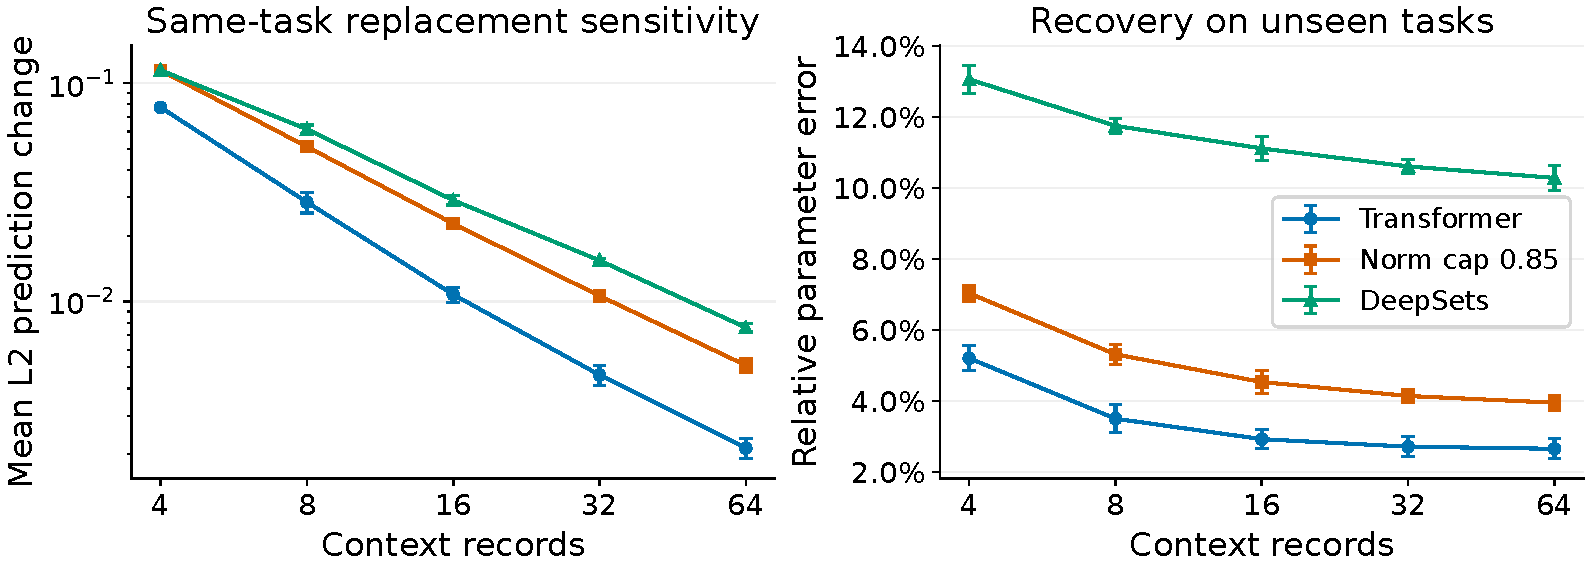
\includegraphics[width=.97\textwidth]{results/presentation/architecture.pdf}
\end{center}
\vspace{-1mm}
\small At \(m=64\), the original Transformer has
\(\Delta=0.00213\) and relative recovery error \(2.65\%\).
\vspace{1mm}

\small{\color{teal}The true task stays fixed, so a small response is compatible with accuracy.}
\source{Experiment D. Four valid same-task replacements per task and length.
The mean curves do not certify worst-case \(1/m\) scaling.}
\note{Target time 45 seconds, cumulative 13:05.
The replacement here comes from the same task, so the correct parameters
stay fixed. Both average prediction change and recovery error decrease
with context length. At length 64, the original Transformer changes by
about 0.00213 and has 2.65 percent relative error. It does best among
these three models under the shared schedule. These are sampled averages,
not a certificate of worst-case inverse-length scaling. Stable, accurate
behavior on ordinary contexts leaves open what happens when information
is nearly redundant.}
\end{frame}

\begin{frame}{Nearly redundant contexts are harder to recover}
\begin{center}
\begin{tabular}{lccc}
\toprule
Context, \(m=16\)&Unique costs?&Minimum Gram eigenvalue&TF error\\
\midrule
Well-conditioned&Yes&\(0.03257\)&\(2.90\%\)\\[2mm]
Nearly redundant&Yes&\(3.72\times10^{-6}\)&\(13.65\%\)\\
\bottomrule
\end{tabular}
\end{center}
\vspace{2mm}
\small Same length \(m=16\) and matched mean demand; different output spreads.
\vspace{2mm}
\begin{itemize}
\setlength{\itemsep}{3mm}
\item \textbf{Identifiability:} do the observations uniquely determine the parameters?
\item \textbf{Conditioning:} how strongly does the whole context constrain each direction?
\end{itemize}
\vspace{3mm}
{\color{teal}Conditioning concerns the context. Next we isolate one record's importance.}
\source{Experiment F. Seed means. The eigenvalue is the minimum across
generator-specific interior Gram matrices normalized by total context size.
Backup C gives all regimes.}
\note{Target time 45 seconds, cumulative 13:50.
Both designs have sixteen records and matched mean demand, but different
output spreads. Both uniquely identify the noiseless costs. Yet the
near-redundant design has a tiny minimum Gram eigenvalue and much larger
Transformer error: 13.65 rather than 2.90 percent. Identifiability asks
whether an answer is unique. Conditioning asks how well the context
constrains each direction. Next we move from whole-context conditioning
to an individual record's leverage, and measure model sensitivity to
a fixed edit.}
\end{frame}

\begin{frame}{The same edit produces a larger response at high leverage}
\begin{columns}[c,onlytextwidth]
\column{.68\textwidth}
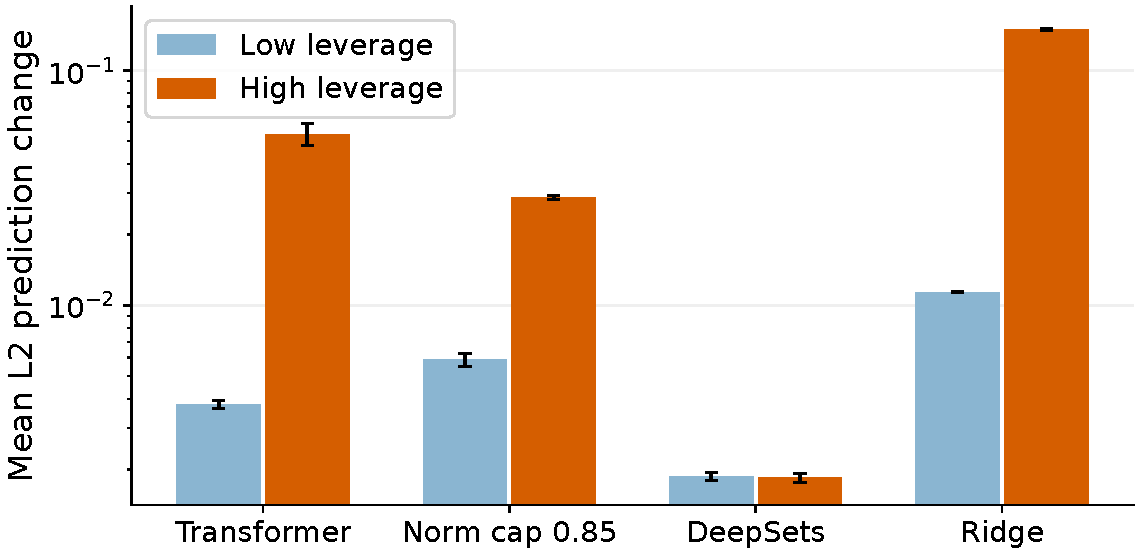
\includegraphics[width=\linewidth]{results/presentation/matched_response.pdf}
\column{.29\textwidth}
\small
\textbf{Leverage:} focal record's importance in the design.

\vspace{2mm}
\textbf{Sensitivity:} measured prediction change.

\vspace{2mm}
Fixed record and \(0.02\) edit.
Different backgrounds.

\vspace{2mm}
High / low response:
\[
\text{Transformer}:14.1\times
\]
\[
\text{Ridge}:13.1\times
\]
\end{columns}
\vspace{2mm}
\small Artificial price edits need not satisfy the original noiseless KKT system.

\vspace{1mm}
{\color{teal}\small Next: valid different-task records test whether response is sufficient.}
\source{Experiment G. Price edit from \(\lambda-0.01\) to \(\lambda+0.01\).
The true task stays fixed. Mean focal hat leverage: 0.999 versus 0.133.}
\note{Target time 50 seconds, cumulative 14:40.
We keep the focal record and price displacement fixed and change the
background. High leverage means the focal record supplies information
the rest provides weakly. Transformer response is 14.1 times larger
there; ridge's ratio is 13.1. Leverage describes the design, while
sensitivity describes the estimator's actual output change. The artificial
price edit can violate the original noiseless KKT equations even though
the true task stays fixed. It demonstrates information-dependent response.
Is that response sufficient when the task really changes? We now return
to the valid identifying pair.}
\end{frame}

\begin{frame}{On the identifying pair, the response remains incomplete}
\begin{columns}[c,onlytextwidth]
\column{.68\textwidth}
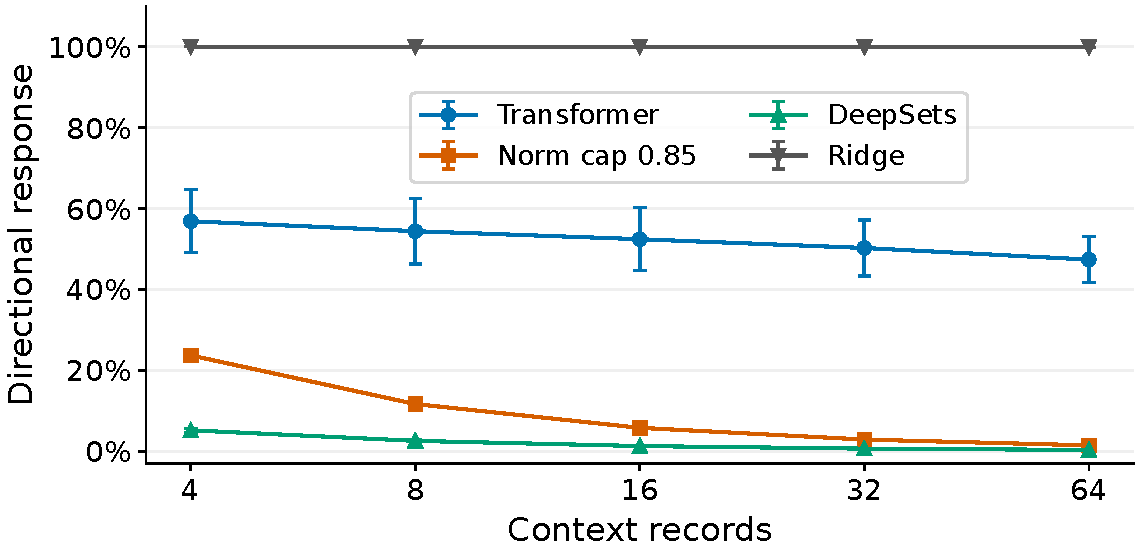
\includegraphics[width=\linewidth]{results/presentation/identifying_response.pdf}
\column{.29\textwidth}
\small
The valid pair from slide 12.

At \(m=64\):
\[
r_{\rm TF}=47.4\%
\]
\[
r_{\rm ridge}=99.9\%.
\]
Larger TF endpoint error:
\[
0.432.
\]
\end{columns}
\[
\small r=
\frac{\langle f(S')-f(S),\,\theta'-\theta\rangle}
{\norm{\theta'-\theta}^{2}}.
\]
\source{Experiment G. \(r=1\) means the correct response along the target
direction. Endpoint error is absolute Euclidean parameter error.}
\note{Target time 60 seconds, cumulative 15:40.
This is the valid dispatch pair from slide twelve. Each endpoint uniquely
identifies its different task. A directional response of one means the
predicted difference recovers the correct change along the target direction;
it does not alone guarantee endpoint accuracy. At length 64 the Transformer
recovers 47.4 percent of that difference, while ridge recovers 99.9 percent.
The larger Transformer endpoint error averages 0.432. This is finite-length
under-response, consistent with the qualitative concern of the corollary.
It neither establishes an asymptotic rate nor follows numerically from
the loose C certificate. We can interpret it instead using the
directional recovery inequality on the next slide.}
\end{frame}

\begin{frame}{Directional response bounds recovery error}
% Generated from saved per-checkpoint outputs; absolute parameter units.
\newcommand{\FinalGap}{1.265}
\newcommand{\FinalDirectional}{0.333}
\newcommand{\FinalEuclidean}{0.331}
\newcommand{\FinalObserved}{0.432}

\small For checkpoint \(j\), let \(M_j=\max\{e_{A,j},e_{B,j}\}\).
Projecting error onto the target direction gives
\[
\boxed{M_j\ge \frac D2|1-r_j|.}
\]
Average \emph{after} taking each checkpoint's maximum:
\(\displaystyle\overline M=\frac1J\sum_{j=1}^J M_j,\quad J=3.\)
\begin{center}
\begin{tabular}{lr}
\toprule
Identifying pair at \(m=64\), \(D=\FinalGap\)&Parameter units\\
\midrule
Directional bound \(\frac{D}{2J}\sum_j|1-r_j|\)&\(\FinalDirectional\)\\[1mm]
Euclidean bound \(\frac1{2J}\sum_j(D-\Delta_j)_+\)&\(\FinalEuclidean\)\\[1mm]
Observed \(\overline M=\frac1J\sum_j\max(e_{A,j},e_{B,j})\)&\(\FinalObserved\)\\
\bottomrule
\end{tabular}
\end{center}
{\color{teal}\small The directional metric on slide 17 yields a finite-length error constraint.}
\source{Each bound holds per checkpoint, then averages. Values use unrounded
saved outputs. \(\overline M\) is not the maximum of the two mean errors.
Backup J gives the projection proof and averaging argument.}
\note{Target time 55 seconds, cumulative 16:35.
We can now connect the directional response directly to recovery.
Project the difference between the target change and predicted change
onto the unit target direction. Its magnitude is D times absolute one
minus r. The two endpoint errors must cover that magnitude, so their
maximum is at least half of it. This holds for every checkpoint.
We average the maximum within each checkpoint, not the maximum of
the two mean endpoint errors. The saved outputs give a directional
lower bound of 0.332904, a Euclidean bound of 0.331170, and an observed
mean larger endpoint error of 0.431601. The absolute value must remain
inside the average in general. All three observed r values are below
one, so here it also equals D over two times one minus mean r.
This is a geometric constraint, without the loose C certificate.}
\end{frame}

\section{Conclusion}
\begin{frame}{Three distinct claims and their scope}
\begin{tabular}{p{.19\textwidth}p{.73\textwidth}}
\toprule
Result & What it establishes\\
\midrule
Theorem 1 & An asymptotic architecture-specific \(C/m\) replacement bound.\\[2mm]
Corollary & A worst-case asymptotic recovery limitation on identifying pairs.\\[2mm]
Experiments & Finite-length identifying under-response, measured separately.\\
\bottomrule
\end{tabular}
\par\vspace{4mm}
\small Our contribution connects an architecture audit, valid identifying
task constructions and controlled behavioral tests.
\vspace{2mm}

\small Limits: loose certificate, repeated-record stress cases, three seeds,
two generators and unresolved internal mechanisms.
\source{Li et al. (2023): established stability reasoning for query prediction.
Theorem 2: generic triangle inequality. Our finite experiments do not verify
the worst-case rate or derive errors from the loose certificate.}
\note{Target time 50 seconds, cumulative 17:25.
Theorem one proves an architecture-specific asymptotic rate. The corollary
turns it into a worst-case recovery restriction for an identifying family.
The experiments separately measure finite-length under-response. They do
not verify the worst-case rate or derive the errors from our loose
certificate. The project connects an adaptation of established stability
reasoning, a valid identifying construction and controlled behavioral
tests. The triangle inequality is generic. Repeated-record stress cases,
three seeds, two generators and unresolved internal mechanisms limit the
claims. Fixed-compute task-count gains also remain inconclusive.}
\end{frame}

\begin{frame}{Information-dependent sensitivity and recovery}
\begin{enumerate}
\setlength{\itemsep}{5mm}
\item A long context can leave one record responsible for a whole parameter direction.
\item Stability bounds response. Identifiability specifies whether a unique answer exists.
The corollary shows a worst-case recovery limitation.
\item The trained Transformer responds to context information,
but its identifying response can remain insufficient.
\end{enumerate}
\vspace{6mm}
{\color{teal}\large\bfseries Information-dependent sensitivity does not guarantee sufficient recovery.}
\note{Target time 35 seconds, cumulative 18:00.
Return to the line example. Many repeated records do not replace
the one observation that determines the slope. The two theorems
compare an architectural response ceiling with the response
required to recover different truths. The experiments show
information-dependent responsiveness, together with incomplete
recovery on the identifying pair. Information-dependent sensitivity does not guarantee sufficient recovery.
That is the final takeaway. The asymptotic corollary and finite-length
observations support distinct parts of this statement.}
\end{frame}

\appendix
\setbeamertemplate{footline}{\hspace{8mm}\textcolor{muted}{\scriptsize Backup}\hfill
\textcolor{muted}{\scriptsize Fei Zhang\quad CS 886}\hspace{8mm}\vspace{3mm}}

\begin{frame}[noframenumbering]{Backup A. Integrating the softmax Jacobian}
\small
\setlength{\abovedisplayskip}{3pt}
\setlength{\belowdisplayskip}{3pt}
\setlength{\abovedisplayshortskip}{2pt}
\setlength{\belowdisplayshortskip}{2pt}
Let \(Q_0,K_0,V_0\) bound query, key and value norms, and set
\[
c_q=\|W_Q\|K_0/\sqrt{d_k},\qquad
c_k=Q_0\|W_K\|/\sqrt{d_k}.
\]
For \(s_i(t)=s_i'+t(s_i-s_i')\), \(p_i(t)=\operatorname{softmax}(s_i(t))\),
every score remains in \([-B,B]\). Thus
\[
p_i-p_i'=\int_0^1J(p_i(t))(s_i-s_i')\,dt,
\]
\[
\begin{aligned}
\|p_i-p_i'\|_1
&\le\int_0^1\sum_j2p_{ij}(t)|s_{ij}-s_{ij}'|\,dt\\
&\le\frac{2e^{2B}}m\sum_j(c_qe_i+c_ke_j)
=2e^{2B}(c_qe_i+c_k\bar e).
\end{aligned}
\]
One head therefore has
\[
\alpha=2V_0e^{2B}c_q,\qquad
\beta=e^{2B}\|W_V\|+2V_0e^{2B}c_k.
\]
\source{For multihead attention, sum head bounds and multiply by the fixed
output-projection norm. All constants depend on fixed maps and state bounds,
not on \(m\).}
\end{frame}
\begin{frame}[noframenumbering]{Backup B. LayerNorm derivative bound}
\small
Let \(P\) center a width-\(p\) row and set
\[
g(z)=\frac{z}{(\|z\|_2^2/p+\eta)^{1/2}},\qquad \eta>0.
\]
The derivative eigenvalues are
\[
\lambda_{\rm tangential}
 =(\|z\|_2^2/p+\eta)^{-1/2},
\qquad
\lambda_{\rm radial}
 =\eta(\|z\|_2^2/p+\eta)^{-3/2}.
\]
Both are at most \(1/\sqrt{\eta}\), and \(\|P\|=1\).
\[
\mathrm{LN}(h)=\operatorname{diag}(\gamma)\,g(Ph)+\beta
\quad\Longrightarrow\quad
L_{\rm LN}\le\frac{\|\gamma\|_\infty}{\sqrt{\eta}}.
\]
\source{Applies to the implemented post-residual LayerNorm with \(\eta=10^{-5}\).}
\end{frame}

\begin{frame}[noframenumbering]{Backup C. All context-information regimes}
\begin{center}
\begin{tabular}{lrrr}
\toprule
Context at \(m=16\)&Minimum Gram eigenvalue&Set diameter&TF error\\
\midrule
Well-conditioned&\(0.03257\)&0&2.90\%\\
Nearly redundant&\(3.72\times10^{-6}\)&0&13.65\%\\
Mixed&\(0.02429\)&0&3.72\%\\
Boundary-heavy&0&1.056&17.64\%\\
\bottomrule
\end{tabular}
\end{center}
\vspace{4mm}
\[
H_i=\frac1m\sum_{t:\,s_{it}=\mathrm{int}}u_{it}u_{it}^{\top},
\qquad u_{it}=(1,x_{it})^\top.
\]
\small The eigenvalue is \(\min_i\lambda_{\min}(H_i)\).
Interior contexts share mean demand; their output spreads differ.
\source{Experiment F. Diameter refers to the boxed KKT-admissible parameter set. Values are seed means.}
\end{frame}

\begin{frame}[noframenumbering]{Backup D. Task-count and training-budget controls}
\begin{center}
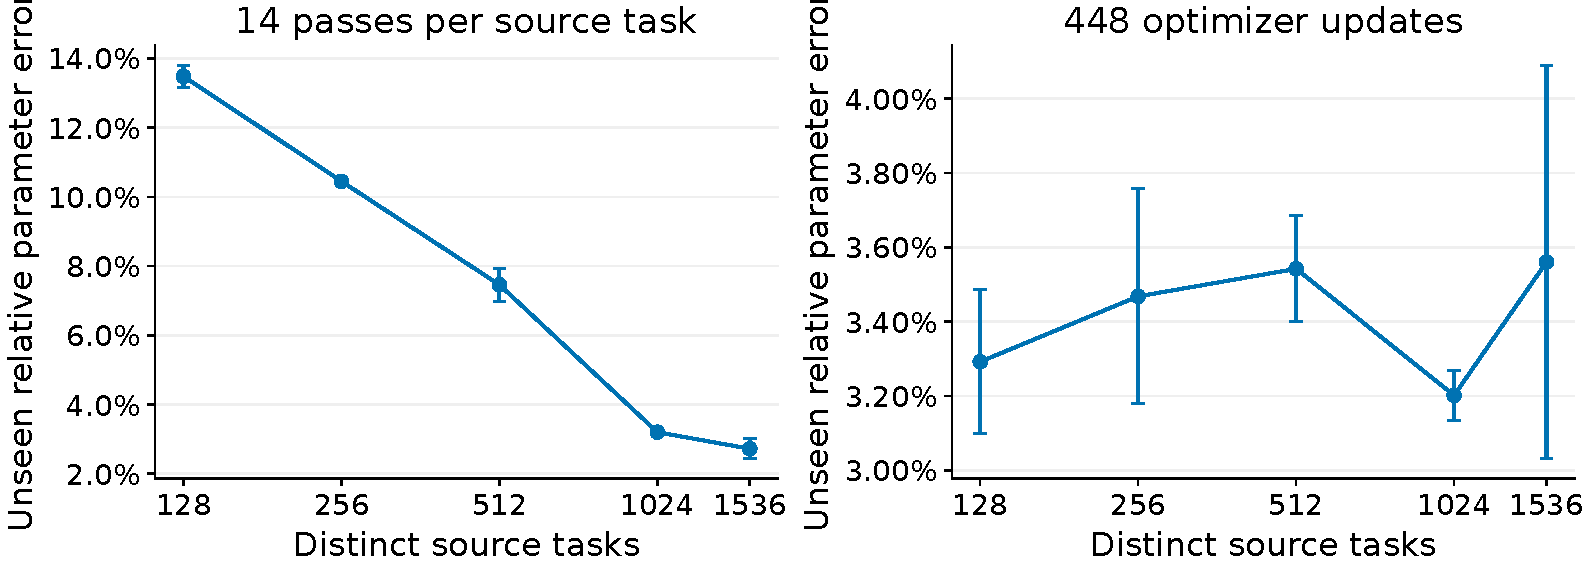
\includegraphics[width=.97\textwidth]{results/presentation/transfer.pdf}
\end{center}
\small The equal-pass sweep spends 56--672 updates as source-task count grows.

\source{Experiment E, evaluation context length 32. Under 448 updates, target error is nonmonotonic across task counts.}
\end{frame}

\begin{frame}[noframenumbering]{Backup E. Information spread across multiple records}
\begin{center}
\begin{tabular}{rrrr}
\toprule
Identifying records \(k\)&TF direction recovered&Largest path step&Larger TF error\\
\midrule
1&50.0\%&0.301&0.281\\
2&52.3\%&0.206&0.272\\
4&53.8\%&0.128&0.266\\
8&54.7\%&0.074&0.262\\
\bottomrule
\end{tabular}
\end{center}
\vspace{4mm}
\small 192 valid task pairs, \(m=64\), target separation 0.6 and focal
price difference 0.09.

\vspace{3mm}
Telescoping a bounded-input path gives
\[
\Delta\le\frac{kC}{m},\qquad
\max(e_A,e_B)\ge\frac12(D-kC/m)_+.
\]
\source{Combine telescoping with Theorem 2. Assumptions and the conditional
asymptotic consequence are on the next backup page.
Completed follow-up. Intermediate price mixtures on the path can be inconsistent with a single noiseless task.}
\end{frame}

\begin{frame}[noframenumbering]{Backup E (continued). Sublinear identifying replacements}
\small
Assume a valid context family for all sufficiently large \(m\):
\begin{itemize}
\setlength{\itemsep}{2mm}
\item Both length-\(m\) endpoints identify their own fixed tasks, with \(D>0\) fixed.
\item They differ in at most \(k_m\) records, with \(k_m=o(m)\).
\item One fixed encoder and a single finite \(C\), independent of \(m\), obey
the replacement bound at every step of a bounded-input replacement path.
\end{itemize}
Then telescoping and Theorem 2 give
\[
\max\{e_A^{(m)},e_B^{(m)}\}\ge
\frac12(D-k_mC/m)_+,
\]
and therefore
\[
\liminf_{m\to\infty}\max\{e_A^{(m)},e_B^{(m)}\}\ge D/2.
\]
\source{Conditional on such an identifying family. Intermediate contexts need
not share one valid noiseless task, but every path step must lie in the
uniform stability domain. Fixed-\(m\) experiments do not establish this limit.}
\end{frame}

\begin{frame}[noframenumbering]{Backup F. Independent noise on every context price}
\begin{center}
\begin{tabular}{lrr}
\toprule
Context at noise SD \(0.04\)&Transformer error&Ridge error\\
\midrule
Well-conditioned&3.87\%&2.39\%\\
Nearly redundant&13.67\%&15.28\%\\
Boundary-heavy&17.41\%&15.50\%\\
\bottomrule
\end{tabular}
\end{center}
\vspace{5mm}
\begin{itemize}
\item Gaussian noise changes prices while dispatch and status stay exact.
\item Ridge uses noisy validation tasks and clipping to the cost box.
\item The frozen Transformer was trained on clean contexts.
\end{itemize}
\source{Completed follow-up. Three seeds, four noise draws per task, length 16.}
\end{frame}

\begin{frame}[noframenumbering]{Backup G. Supporting task-level transfer bound}
\small
For IID source tasks and a fixed hypothesis class, define
\[
L_\theta(f)=\mathbb E_{S\sim P_\theta^m}
  \left[\frac14\sum_{j=1}^{4}
    \left(\frac{f_j(S)-\theta_j}{\mathrm{span}_j}\right)^2\right].
\]
With an \(\varepsilon\)-cover of the task-risk functions in sup norm of
size \(N_\varepsilon\), with probability at least \(1-\delta\),
\[
\left|\mathbb E_\theta L_\theta(f)-\frac1T\sum_{t=1}^{T}L_{\theta_t}(f)\right|
\le2\varepsilon+
\sqrt{\frac{\log(2N_\varepsilon/\delta)}{2T}}.
\]
Hoeffding at each center, a union bound, and two approximation terms prove the claim.
\source{Standard uniform convergence argument. The class and same-distribution assumptions determine its scope.}
\end{frame}

\begin{frame}[noframenumbering]{Backup H. References and reproducibility}
\footnotesize
\begin{itemize}
\setlength{\itemsep}{3mm}
\item Li, Ildiz, Papailiopoulos and Oymak (2023).
\emph{Transformers as Algorithms}. ICML.
\href{https://proceedings.mlr.press/v202/li23l.html}{Paper}
\item Keshavarz, Wang and Boyd (2011).
\emph{Imputing a Convex Objective Function}. IEEE MSC.
\item Aky\"urek et al.\ (2023).
\emph{What Learning Algorithm Is In-Context Learning?} ICLR.
\item Chakraborty, Luo and Barber (2026).
\emph{Stability and Accuracy Trade-offs in Statistical Estimation}.
\end{itemize}
\vspace{4mm}
\href{https://github.com/feizhanguwaterloo/Stability-and-Information-Sensitivity-in-Transformer-In-Context-Inverse-Learning}
{\textcolor{teal}{Project repository with code, tests, configurations, results and report source}}
\end{frame}

\begin{frame}[noframenumbering]{Backup I. Leverage and measurement perturbations}
\small
For generator \(i\), let \(u_{it}=(1,x_{it})^\top\) and
\[
H_i=\frac1m\sum_{t:s_{it}=\mathrm{int}}u_{it}u_{it}^{\top}.
\]
On the all-interior matched designs, the focal last record has leverage
\[
h_{i,m}=\frac1m\,u_{i,m}^{\top}H_i^\dagger u_{i,m},
\qquad
h_{\mathrm{focal}}=\max_{i\in\{1,2\}}h_{i,m}.
\]
This equals the focal diagonal of the regression hat matrix for each unit,
followed by the maximum across units.
\vspace{3mm}

Implementation: \texttt{hat\_leverage}, \texttt{src/leverage.py},
uses \texttt{pinv(gram, rcond=1e-12)} and divides by \(m\).
\vspace{3mm}

Price edits preserve dispatch, status and the true task, but can violate
\(\lambda=a_i+b_ix_i\). Slide 17 uses a separate, valid different-task pair.
\source{The formula matches the all-interior contexts used by this intervention.
Leverage describes design geometry; sensitivity describes model output.}
\end{frame}

\begin{frame}[noframenumbering]{Backup J. Directional recovery proof and checkpoint averages}
\small
Let \(\delta=\theta_B-\theta_A\), \(D=\|\delta\|_2>0\), \(u=\delta/D\),
\(v_j=f_j(S_B)-f_j(S_A)\), and \(r_j=\langle v_j,\delta\rangle/D^2\).
Writing \(\varepsilon_{A,j}=f_j(S_A)-\theta_A\) and similarly for B,
\[
D|1-r_j|
=|u^\top(\delta-v_j)|
=|u^\top(\varepsilon_{A,j}-\varepsilon_{B,j})|
\le e_{A,j}+e_{B,j}\le2M_j.
\]
Thus
\[
\overline M=\frac1J\sum_j M_j
\ge\frac D{2J}\sum_j|1-r_j|
\ge\frac D2|1-\overline r|.
\]
The last step is Jensen's inequality; the middle bound retains all checkpoint
variation. In our three outputs \(r_j<1\), so both directional expressions agree.
\vspace{2mm}

The Euclidean bound also averages checkpointwise:
\[
\overline M\ge\frac1{2J}\sum_j(D-\Delta_j)_+
\ge\frac12(D-\overline\Delta)_+.
\]
\source{Here \(e_{A,j}=\|\varepsilon_{A,j}\|_2\) and
\(M_j=\max(e_{A,j},e_{B,j})\).
All errors are absolute Euclidean parameter errors, not relative errors.}
\end{frame}
\end{document}
